\documentclass[11pt,a4paper]{article}

\usepackage[utf8]{inputenc}
\usepackage[T1]{fontenc}
\usepackage[english]{babel}
\usepackage{geometry}
\geometry{a4paper, margin=2.5cm}
\usepackage{graphicx}
\usepackage{float}
\usepackage{booktabs}
\usepackage{hyperref}
\usepackage{enumitem}
\usepackage{amsmath}
\usepackage{setspace}
\usepackage{tikz}
\usetikzlibrary{shapes.geometric, arrows.meta, positioning, fit, backgrounds}
\setstretch{1.15}

\title{\textbf{A Fully Automated Distributed Pipeline for Water Meter Reading: Integrating YOLO-Based ROI Detection and CNN-Based Inference}}
\author{Anass Ouzaouit \\ \textit{Supervised by: Prof. Abdessadek Aaroud} \\ Master's in Business Intelligence and Big Data Analytics}
\date{\today}

\begin{document}

\maketitle

\begin{abstract}
Automated Meter Reading (AMR) is an important component of smart infrastructure, enabling utility providers to digitize meter readings without replacing existing hardware. However, many practical edge-based solutions still depend on manual Region of Interest (ROI) configuration, which limits scalability and increases deployment effort. This paper proposes a fully automated distributed AMR pipeline that removes this bottleneck through a two-stage architecture: a lightweight YOLOv8n detector automatically localizes the meter digit strip, and a custom CNN classifies segmented digits on a separate inference node through TCP communication. 

To organize the discussion, the paper follows the LBC matrix: \textit{Literature} reviews prior AMR approaches and identifies the limitations of manual-ROI workflows, \textit{Business need} motivates the need for an autonomous and scalable system, and \textit{Contribution} presents the proposed distributed architecture and its experimental validation. The model achieves a 100\% ROI detection success rate on the local test set and 99.00\% hold-out accuracy for digit classification. End-to-end evaluation on an independent dataset reaches a 72.00\% exact full-reading match, showing that the proposed system is effective but still limited by segmentation errors under difficult lighting conditions.
\end{abstract}

\textbf{Keywords:} Automated Meter Reading, YOLOv8, CNN, Distributed Inference, Edge Computing, ROI Detection.

\vspace{1em}

\section{Introduction}
The growth of smart cities and connected infrastructure has increased the need for reliable and low-cost methods of collecting utility data. Automated Meter Reading (AMR) addresses this need by extracting numeric readings from analog water, gas, or electricity meters using computer vision rather than manual inspection. In practice, however, many systems still depend on human-assisted setup, especially when the digit area must be manually defined before inference can begin.

This work is structured according to the \textbf{LBC matrix}, which separates the study into three parts. The \textbf{L}iterature axis summarizes prior work and highlights current technical limitations, the \textbf{B}usiness axis defines the operational need for a scalable and autonomous solution, and the \textbf{C}ontribution axis presents the proposed distributed pipeline and its evaluation.

\section{L-Axis: Literature and State of the Art}

\subsection{Early AMR Approaches}
Traditional AMR systems often relied on classical image processing methods such as thresholding, edge detection, contour extraction, and morphological filtering to identify the meter window or digit strip. These methods are computationally efficient, but they are highly sensitive to illumination changes, shadows, reflections, camera motion, and meter degradation. As a result, they tend to work only under controlled conditions.

\subsection{Deep Learning for Meter Reading}
Recent progress in deep learning has significantly improved object detection and recognition tasks. In particular, YOLO-based detectors offer a strong trade-off between speed and accuracy, which makes them suitable for real-time or edge-oriented applications. For meter reading, detection models can be used to localize the ROI automatically, while CNN-based classifiers can recognize individual digits after segmentation.

\subsection{Relevant Existing Work}
Several recent studies have demonstrated the effectiveness of learning-based AMR systems. Laroca et al.~\cite{laroca2019} introduced a CNN-based pipeline for automatic meter reading, showing that deep models can replace hand-crafted feature engineering in practical meter analysis. In a later study, Laroca et al.~\cite{laroca2021} proposed a robust image-based AMR system for unconstrained scenarios, highlighting the advantages of deep learning for meter localization and reading under real-world conditions. Related work on analog dial meters also explored deep learning for automatic reading, including YOLO-based detection and regression-oriented estimation strategies for unconstrained dial-meter scenarios~\cite{laroca2020dial}. Together, these studies confirm the value of data-driven approaches while also motivating lighter and more deployment-oriented architectures.

\subsection{Limitations of Manual ROI Setups}
Despite these advances, some practical edge deployments still require manual ROI configuration. In such workflows, the user must draw the digit strip manually during installation, and the system becomes fragile if the camera position changes later. This limitation reduces deployment scalability and increases maintenance cost. The legacy AI-on-the-Edge workflow is a representative example of this issue, since it relies on human-defined bounding regions instead of fully automatic localization.

\begin{figure}[H]
    \centering
    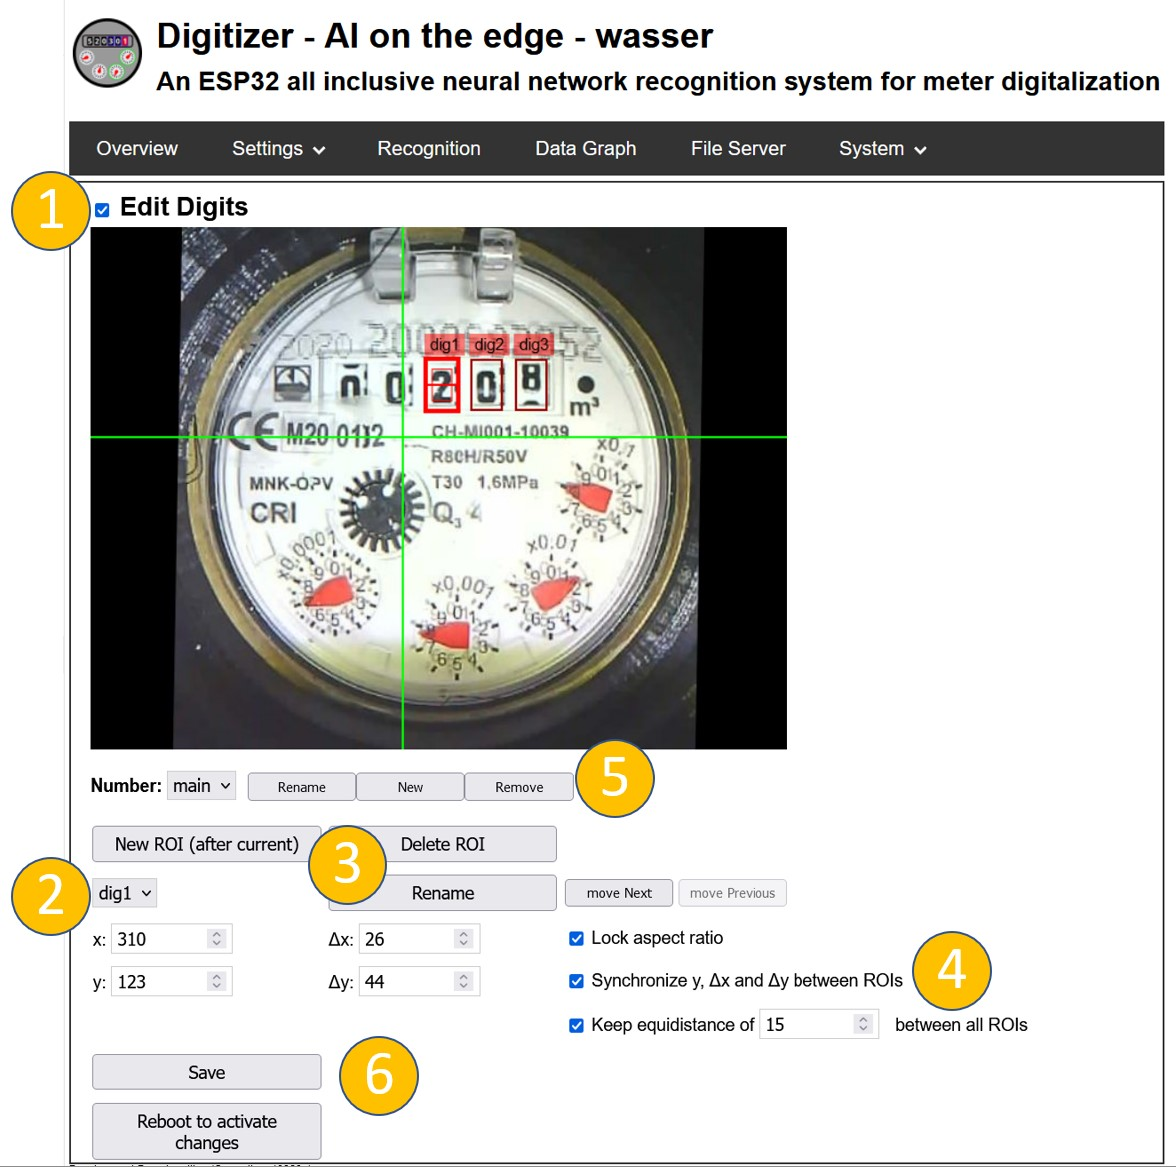
\includegraphics[width=0.6\textwidth]{figures/jomjol roi .png}
    \caption{Manual ROI configuration in a legacy edge workflow, illustrating the deployment bottleneck addressed in this work.}
\end{figure}

\section{B-Axis: Business Need and Problem Statement}

\subsection{Scalability Requirement}
From an industrial perspective, large-scale AMR deployment must minimize human intervention. A utility provider managing thousands of endpoints cannot afford repeated manual setup or recalibration for each camera installation. Therefore, the system must detect the reading region automatically and remain robust to small shifts in camera angle, distance, or alignment.

\subsection{Problem Statement}
The main question addressed in this paper is:
\begin{quote}
How can manual ROI configuration be eliminated in edge-based AMR systems to build a fully autonomous and scalable reading pipeline?
\end{quote}

\subsection{Operational Requirements}
To satisfy this need, the proposed system should:
\begin{enumerate}[label=\arabic*.]
    \item Detect the digit region automatically without manual bounding-box setup.
    \item Read individual characters accurately after cropping and segmentation.
    \item Operate in a distributed mode where image acquisition and ROI localization can be separated from digit classification.
    \item Remain lightweight enough to support practical deployment on constrained hardware.
\end{enumerate}

\section{C-Axis: Contribution and System Design}

\subsection{Overview of the Proposed Pipeline}
To address the problem, we propose a distributed AMR architecture composed of two communicating nodes. Machine A performs image acquisition and ROI detection using a lightweight YOLOv8n model. Machine B receives the cropped ROI over a TCP socket, segments the digits using classical image-processing steps, and classifies them with a custom CNN. This separation reduces the burden on the acquisition node while preserving modularity and flexibility.

\subsection{Distributed Architecture}
The system is organized as follows:
\begin{itemize}
    \item \textbf{Machine A (Client):} captures the meter image, detects the ROI with YOLOv8n, crops the digit strip, and transmits only the cropped image data to the second node.
    \item \textbf{Machine B (Server):} receives the cropped ROI, performs digit segmentation using OpenCV-based preprocessing, classifies each digit with a CNN, and reconstructs the final reading.
\end{itemize}

\begin{figure}[H]
    \centering
    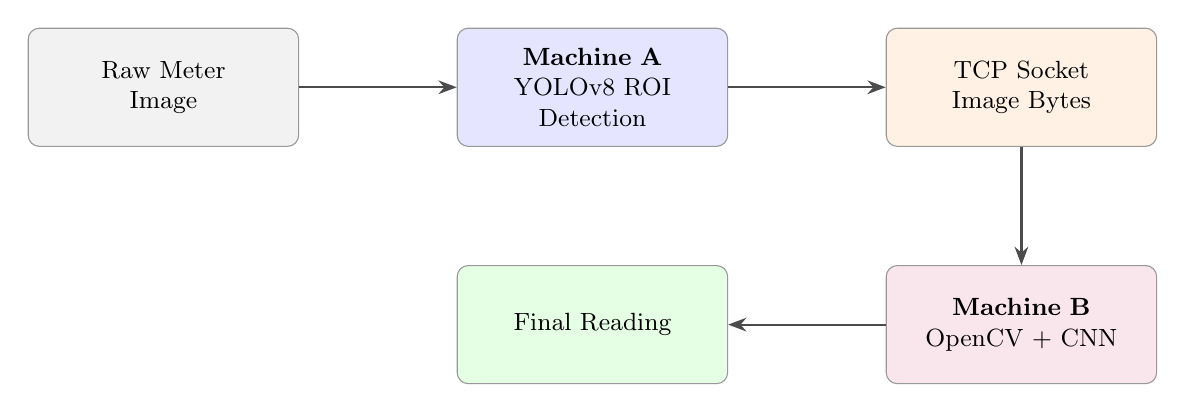
\begin{tikzpicture}[
        node distance=1.5cm and 2cm,
        box/.style={rectangle, draw=black!40, rounded corners, fill=blue!5, text width=3.2cm, align=center, minimum height=1.5cm, font=\small},
        arrow/.style={-{Stealth}, thick, draw=black!70}
    ]
    \node[box, fill=gray!10] (meter) {Raw Meter\\Image};
    \node[box, right=of meter, fill=blue!10] (machA) {\textbf{Machine A}\\YOLOv8 ROI Detection};
    \node[box, right=of machA, fill=orange!10] (socket) {TCP Socket\\Image Bytes};
    \node[box, below=of socket, fill=purple!10] (machB) {\textbf{Machine B}\\OpenCV + CNN};
    \node[box, left=of machB, fill=green!10] (result) {Final Reading};

    \draw[arrow] (meter) -- (machA);
    \draw[arrow] (machA) -- (socket);
    \draw[arrow] (socket) -- (machB);
    \draw[arrow] (machB) -- (result);
    \end{tikzpicture}
    \caption{Proposed distributed AMR pipeline with automatic ROI detection and remote digit inference.}
\end{figure}

\subsection{Automatic ROI Detection with YOLOv8}
A YOLOv8n model was trained to detect a single class, namely \textit{counter\_roi}, using data adapted from the UFPR-AMR dataset. Reducing the detection problem to a single class simplifies training and improves convergence while preserving robustness in unconstrained scenes. The model achieved the following validation results:
\begin{itemize}
    \item \textbf{mAP@50:} 99.34\%
    \item \textbf{mAP@50-95:} 75.62\%
\end{itemize}

\begin{figure}[H]
    \centering
    \includegraphics[width=0.3\textwidth]{figures/yolo crop.png}
    \caption{Example of autonomous ROI extraction using YOLOv8n. The detector isolates the digit strip without manual configuration.}
\end{figure}

\subsection{Digit Segmentation and CNN Classification}
After ROI extraction, the cropped image is sent to Machine B for digit segmentation and classification. The segmentation pipeline uses a deterministic sequence of operations:
\begin{enumerate}
    \item \textbf{Grayscale conversion and Gaussian blur:} reduce color noise and suppress local artifacts.
    \item \textbf{Otsu thresholding:} binarize the ROI and emphasize the digit shapes.
    \item \textbf{Morphological operations:} improve character continuity and remove small noisy components.
    \item \textbf{Vertical projection:} identify blank columns between digits and extract character regions.
\end{enumerate}

\begin{figure}[H]
    \centering
    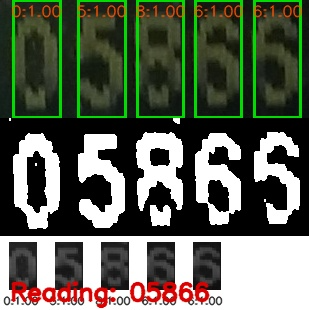
\includegraphics[width=0.6\textwidth]{figures/cnn detection.png}
    \caption{Digit segmentation and CNN inference on Machine B using the reading ``05866'' as an example.}
\end{figure}

Each segmented digit is resized to a 20$\times$32 RGB image and fed to a custom TensorFlow/Keras CNN. The classifier predicts 11 classes: digits 0 to 9, plus an additional \textit{N/NaN} class for unreadable or absent characters.

\subsection{Training Data and Model Setup}
The CNN was trained on 9,960 digit crops extracted from UFPR-AMR annotations. The dataset was split into 7,968 training samples and 1,992 hold-out test samples. Training was performed on raw pixel values without normalization by 255, and early stopping was used to avoid overfitting. The best model was recovered at epoch 104, while training stopped at epoch 124.

\begin{figure}[H]
    \centering
    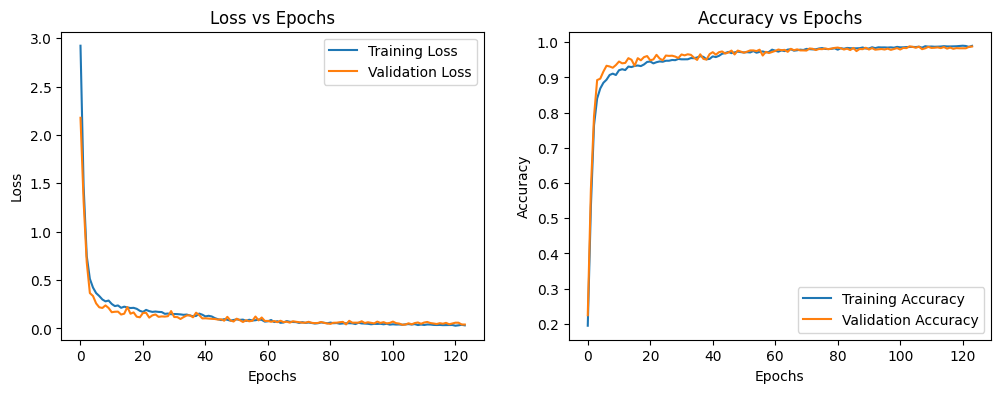
\includegraphics[width=0.9\textwidth]{figures/loss and accuracy.png}
    \caption{Training curves for the CNN classifier over 124 epochs. The final hold-out accuracy reached 99.00\%.}
\end{figure}

\section{Experimental Validation}

\subsection{Evaluation Protocol}
The complete pipeline was evaluated on an independent local test set of 50 meter images. The evaluation measured both component-level performance and end-to-end reading quality.

\subsection{Component-Level Performance}
On the local set, the YOLO detector successfully localized the ROI in all 50 images, yielding a 100\% detection success rate. The average confidence score was 80.76\%, and the average IoU was 88.66\%. The CNN classifier achieved 99.00\% accuracy on the hold-out digit test set, with macro and weighted F1 scores both equal to 0.99.

\subsection{End-to-End Results}
The final reading performance is summarized in Table~\ref{tab:endtoend}.

\begin{table}[H]
\centering
\begin{tabular}{lc}
\toprule
\textbf{Metric} & \textbf{Performance} \\
\midrule
Exact full-reading match & 72.00\% (36/50) \\
Correct text-length prediction & 76.00\% (38/50) \\
\bottomrule
\end{tabular}
\caption{End-to-end evaluation on 50 meter images.}
\label{tab:endtoend}
\end{table}

\subsection{Error Analysis}
The gap between component-level accuracy and end-to-end reading accuracy is mainly caused by segmentation failures. In particular, strong reflections and glare on the glass surface can reduce the visibility of spaces between digits. When this occurs, the vertical projection step may merge multiple digits into one region or miss some characters entirely. In one representative failure case, the reading ``21931'' was incorrectly reconstructed as ``43'' because the segmentation stage under-detected the character boundaries. Since the CNN performs well on isolated digits, the main weakness lies in the boundary extraction stage rather than the classifier itself.

\begin{figure}[H]
    \centering
    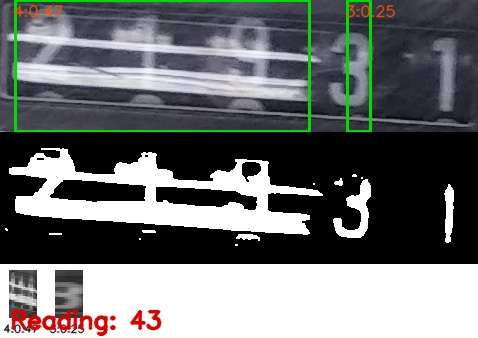
\includegraphics[width=0.8\textwidth]{figures/cnn error.jpg}
    \caption{Example of under-segmentation caused by glare and reflection, leading to an incorrect full reading.}
\end{figure}

\subsection{System Limitations}
While the proposed system demonstrates strong performance on the UFPR-AMR dataset distribution, it exhibits several generalization limitations consistent with the domain shift problem in computer vision:
\begin{itemize}
    \item \textbf{Novel Meter Types:} The YOLOv8 detector was trained exclusively on UFPR-AMR meters and struggles to generalize to completely unseen meter styles, colors, or shapes.
    \item \textbf{Extreme Rotations:} The model relies on standard axis-aligned bounding boxes and limited rotation augmentation during training, leading to failures on heavily rotated images.
    \item \textbf{Otsu Segmentation Assumptions:} The classical Otsu thresholding step assumes a bimodal grayscale distribution (e.g., dark digits on a light background). This assumption breaks down when applied to colored or heavily stylized meter dials, causing downstream segmentation failures.
\end{itemize}
These findings highlight the trade-off between the high accuracy achieved on in-distribution data and the challenges of zero-shot generalization to unconstrained real-world environments.

\section{Benchmark and Positioning}

To position the proposed method with respect to prior work, Table~\ref{tab:benchmark} compares our architecture against existing AMR solutions across key deployment dimensions.

\begin{table}[H]
\centering
\begin{tabular}{@{}p{3.8cm} p{3.8cm} p{3.6cm} c c@{}}
\toprule
\textbf{System / Approach} & \textbf{ROI Localization} & \textbf{Digit Recognition} & \textbf{Autonomy} & \textbf{Scalability} \\
\midrule
Legacy Edge (Jomjol \cite{jomjol}) & Manual via web UI & TFLite-based CNN & Low & Low \\
Traditional CV Pipelines & Rule-based / contours & OCR / heuristic reading & Medium & Medium \\
Laroca et al. \cite{laroca2021} & Deep-learning-based localization & Deep learning reading pipeline & High & Medium \\
Salomon et al. \cite{laroca2020dial} & YOLOv4-based detection & AngReg-based reading & High & Medium \\
\midrule
\textbf{Proposed System} & \textbf{Automatic (YOLOv8)} & \textbf{Custom CNN (99\%)} & \textbf{High} & \textbf{High} \\
\bottomrule
\end{tabular}
\caption{Benchmark comparing the proposed distributed architecture against representative AMR solutions.}
\label{tab:benchmark}
\end{table}

As shown in the benchmark, classical pipelines remain sensitive to environmental variation, while manual-ROI edge systems do not scale well because they depend on user configuration. Deep-learning-based AMR systems such as that of Laroca et al.~\cite{laroca2021} demonstrate strong robustness and automation, but they are better aligned with centralized or resource-richer deployments than with minimal edge-only setups. The proposed distributed architecture addresses this gap by assigning lightweight ROI detection to the acquisition node and offloading the remaining recognition workload to a second node, thereby combining automation with practical deployment scalability.

\section{Conclusion and Perspectives}
This paper presented a fully automated distributed AMR system that combines YOLO-based ROI detection with CNN-based digit classification. The proposed architecture directly addresses the deployment bottleneck created by manual ROI configuration in existing edge-based workflows. By separating detection and inference across two nodes, the system also offers a practical path toward scalable and modular deployment.

Experimental results show strong component-level performance, with 100\% ROI detection success and 99.00\% digit classification accuracy on the local test set. However, end-to-end performance remains limited by segmentation errors under difficult lighting conditions and generalization challenges on novel meter types. 

Future work should directly address these generalization constraints. To handle extreme rotations, the detection stage could be upgraded to use Oriented Bounding Boxes (OBB) or trained with aggressive affine augmentations. Furthermore, to overcome the limitations of Otsu segmentation and improve resilience against domain shifts (such as colored dials), the deterministic projection-based step should be replaced with a sequence modeling approach—such as a CRNN with CTC loss—or an end-to-end object detector for individual digits. This would eliminate hard segmentation assumptions, improving full-reading accuracy across diverse meter types and reducing sensitivity to glare.

\begin{thebibliography}{99}

\bibitem{ufpr}
A. L. B. de Mello et al., \emph{UFPR-AMR Dataset}. Available: \url{https://web.inf.ufpr.br/vri/databases/ufpr-amr/}

\bibitem{jomjol}
Jomjol, \emph{AI-on-the-edge-device Open Source Repository}. Available: \url{https://github.com/jomjol/AI-on-the-edge-device}

\bibitem{yolov8}
Ultralytics, \emph{YOLOv8 Documentation}. Available: \url{https://docs.ultralytics.com/}

\bibitem{keras}
TensorFlow Team, \emph{TensorFlow and Keras Documentation}. Available: \url{https://www.tensorflow.org/}

\bibitem{laroca2021}
R. Laroca, A. B. Araujo, L. A. Zanlorensi, E. C. de Almeida, and D. Menotti, \emph{Towards Image-based Automatic Meter Reading in Unconstrained Scenarios: A Robust and Efficient Approach}, IEEE Access, vol. 9, pp. 67569--67584, 2021. \url{https://doi.org/10.1109/ACCESS.2021.3077415}

\bibitem{laroca2019}
R. Laroca et al., \emph{Convolutional Neural Networks for Automatic Meter Reading}, Journal of Electronic Imaging, vol. 28, no. 1, 2019. \url{https://doi.org/10.1117/1.JEI.28.1.013023}

\bibitem{laroca2020dial}
R. Laroca et al., \emph{Deep Learning for Image-based Automatic Dial Meter Reading}, arXiv:2005.03106, 2020. \url{https://arxiv.org/abs/2005.03106}

\end{thebibliography}

\end{document}